\documentclass[12pt,a4paper]{article}

% ============ PAQUETES ESENCIALES ============
\usepackage[utf8]{inputenc}
\usepackage[spanish]{babel}
\usepackage{amsmath,amssymb,amsthm}
\usepackage{algorithm,algpseudocode}
\usepackage{graphicx}
\usepackage{booktabs,multirow,longtable,array}
\usepackage{caption,subcaption}
\usepackage{listings,xcolor}
\usepackage{hyperref}
\usepackage{geometry}
\usepackage{float}
\usepackage{pdflscape}
\usepackage{siunitx}
\usepackage{xcolor}

\geometry{margin=2.5cm}

% ============ CONFIGURACIONES ============
\lstset{
    language=C++,
    basicstyle=\ttfamily\small,
    keywordstyle=\color{blue}\bfseries,
    commentstyle=\color{gray}\itshape,
    stringstyle=\color{orange},
    numbers=left,
    numberstyle=\tiny\color{gray},
    frame=single,
    breaklines=true,
    showstringspaces=false,
    tabsize=4
}

\hypersetup{
    colorlinks=true,
    linkcolor=blue,
    citecolor=blue,
    urlcolor=blue,
    pdftitle={Optimizacion y Redes Neuronales - Taller 7},
    pdfauthor={Gregory Uzcategui}
}

% ============ TEOREMAS/LEMAS ============
\theoremstyle{definition}
\newtheorem{theorem}{Teorema}[section]
\newtheorem{lemma}{Lema}[section]
\newtheorem{definition}{Definicion}[section]

% ============ COMANDOS PERSONALIZADOS ============
\newcommand{\norm}[1]{\|#1\|}
\newcommand{\R}{\mathbb{R}}
\newcommand{\vect}[1]{\mathbf{#1}}
\newcommand{\dd}[2]{\frac{\partial #1}{\partial #2}}

% ============ DOCUMENTO ============
\begin{document}

% ---------- PORTADA ----------
\begin{titlepage}
    \centering
    \vspace*{2cm}
    {\Huge\bfseries Optimizaci\'{o}n y Redes Neuronales\\[0.3cm] Entrenamiento de un Aproximador No Lineal mediante Backpropagation\par}
    \vspace{1.5cm}
    {\Large Informe T\'{e}cnico de Implementaci\'{o}n y Resultados\par}
    \vspace{2cm}
    {\Large Autor: Gregory Uzcategui / CI: 27.376.191 \par}
    \vspace{2cm}
    {\large
    \textbf{Stack tecnol\'{o}gico:} C++17 (Eigen 3.4), CMake, Python 3 (pandas, matplotlib)\\[0.5cm]
    \textbf{M\'{e}todo num\'{e}rico:} Backpropagation con Descenso de Gradiente y activaci\'{o}n ReLU\\[0.5cm]
    \textbf{Metodolog\'{i}a de desarrollo:} SDD (Specification-Driven Development) con VSCode + Continue\\[0.5cm]
    \textbf{Problema:} Aproximaci\'{o}n de $f(x) = x^2 + \sin(5x) + \epsilon$ en $[-2, 2]$
    \par}
    \vfill
    {\large \textbf{Octubre 2026}}
\end{titlepage} 

% ---------- RESUMEN ----------
\begin{abstract}
\noindent
La implementaci\'{o}n de una red neuronal de una capa oculta con activaci\'{o}n ReLU para aproximar la funci\'{o}n no lineal $f(x) = x^2 + \sin(5x) + \epsilon$ en el dominio $x \in [-2, 2]$. Se desarroll\'{o} el algoritmo de \textbf{Backpropagation} desde cero en C++17 con Eigen, calculando manualmente los gradientes de la funci\'{o}n de costo MSE respecto a cada peso y sesgo mediante la Regla de la Cadena. Se evaluaron tres tasas de aprendizaje ($\alpha \in \{0.001, 0.01, 0.5\}$) con cinco semillas aleatorias distintas, evidenciando la presencia de \textbf{m\'{i}nimos locales} en el paisaje de optimizaci\'{o}n no convexo. 
\end{abstract}

\tableofcontents
\newpage

% ---------- 1. INTRODUCCION ----------
\section{Introducci\'{o}n}\label{sec:intro}

El entrenamiento de una red neuronal es, en esencia, un problema de \textbf{optimizaci\'{o}n no lineal y no convexa}. En este taller, se construye desde cero una red con una capa oculta para aproximar una funci\'{o}n compleja. El objetivo es comprender c\'{o}mo la informaci\'{o}n fluye hacia adelante (\textit{Forward Pass}) y c\'{o}mo el error se propaga hacia atr\'{a}s (\textit{Backward Pass}) para actualizar los par\'{a}metros del modelo.

\subsection{Metodolog\'{i}a de Desarrollo: SDD con Continue}

El proyecto se desarroll\'{o} siguiendo la metodolog\'{i}a \textbf{Specification-Driven Development (SDD)}, donde cada m\'{o}dulo se implementa a partir de una especificaci\'{o}n formal en Markdown. Se utiliz\'{o} \textbf{VSCode} con la extensi\'{o}n \textbf{Continue} (asistente de IA) para generar el c\'{o}digo a partir de los prompts estructurados.

\subsubsection{Prompt Inicial utilizado con Continue}

El siguiente prompt se utiliz\'{o} como punto de partida para guiar la implementaci\'{o} m\'{o}dulo a m\'{o}dulo:

\begin{lstlisting}[caption={Prompt inicial para Continue en VSCode.}, label={lst:prompt}]
El siguiente documento es sobre el taller 7: Optimizacion y Redes
Neuronales, de la materia computo cientifico, el documento tiene
lineas resaltadas con un codigo de color especifico, amarillo para
palabras y definiciones que no entiendo, rojo para el contenido que
tengo que desarrollar (programar el calculo) que no se como
implementarlo al 100%, necesito una guia clara para aprender y
entender como se hace y verde para los modulos del algoritmo. Las
tecnologias son C++ libreria Eigen y python con matplotlib, pandas
y numpy. C++ motor del calculo, python graficas; mis herramientas
de trabajo son VScode y Continue usando la metodologia spec driven
developed.
\end{lstlisting}

Este prompt permiti\'{o} a la IA:
\begin{itemize}
    \item Identificar las \textbf{zonas amarillas} (conceptos te\'{o}ricos a explicar: ReLU, Backpropagation, M\'{i}nimos Locales).
    \item Desarrollar las \textbf{zonas rojas} (implementaci\'{o}n matem\'{a}tica de los gradientes).
    \item Estructurar las \textbf{zonas verdes} (m\'{o}dulos del algoritmo: \texttt{data\_generator}, \texttt{neural\_network}, \texttt{trainer}).
\end{itemize}

\begin{table}[H]
\centering
\caption{Estructura de especificaciones SDD generadas.}
\label{tab:specs}
\begin{tabular}{@{}llp{7cm}@{}}
\toprule
\textbf{Archivo} & \textbf{M\'{o}dulo} & \textbf{Responsabilidad} \\ \midrule
\texttt{ARCH\_DESIGN.md} & Global & Arquitectura, contratos de datos, stack tecnol\'{o}gico \\
\texttt{spec-001.md} & \texttt{data\_generator} & Generaci\'{o}n de datos $y = x^2 + \sin(5x) + \epsilon$ \\
\texttt{spec-002.md} & \texttt{neural\_network} & Forward/Backward pass con ReLU y MSE \\
\texttt{spec-003.md} & \texttt{trainer} & Bucle de entrenamiento con 5 semillas $\times$ 3 $\alpha$ \\
\texttt{spec-004.md} & \texttt{exportador} & Persistencia de resultados a CSV \\
\texttt{spec-005.md} & \texttt{main.cpp} & Orquestador del pipeline completo \\
\texttt{spec-py.md} & \texttt{visualizar\_nn.py} & Gr\'{a}ficas de convergencia y ajuste \\ \bottomrule
\end{tabular}
\end{table}

\subsection{Justificaci\'{o}n de las Herramientas Tecnol\'{o}gicas}

\begin{itemize}
    \item \textbf{C++ y Eigen 3.4:} Se eligi\'{o} C++ por su alto rendimiento en c\'{a}lculo num\'{e}rico (el entrenamiento requiere miles de iteraciones con multiplicaciones matriciales). Eigen proporciona operaciones vectorizadas SIMD y manejo eficiente de matrices densas, esencial para el c\'{a}lculo de gradientes en lote (\textit{batch}).

    
    \item \textbf{Python (pandas, matplotlib):} Se utiliz\'{o} Python exclusivamente para la fase de post-procesamiento. Separar el c\'{a}lculo pesado (C++) de la visualizaci\'{o}n (Python) es una pr\'{a}ctica est\'{a}ndar. Python permite parsear los CSV generados y generar gr\'{a}ficas de calidad de publicaci\'{o}n (curvas de convergencia, ajuste de la red) con pocas l\'{i}neas de c\'{o}digo.
\end{itemize}

\subsection{Objetivos}
\begin{itemize}
    \item Implementar manualmente el \textbf{Forward Pass} y \textbf{Backward Pass} en C++17 con Eigen.
    \item Aplicar la funci\'{o}n de activaci\'{o}n \textbf{ReLU} en la capa oculta.
    \item Minimizar la funci\'{o}n de costo \textbf{MSE} mediante Descenso de Gradiente.
    \item Analizar el efecto de la \textbf{tasa de aprendizaje} $\alpha \in \{0.001, 0.01, 0.5\}$.
    \item Demostrar la presencia de \textbf{m\'{i}nimos locales} mediante 5 semillas aleatorias.
    \item Visualizar la convergencia y el ajuste de la red mediante Python.
\end{itemize}

% ---------- 2. MARCO TEORICO ----------
\section{Marco Te\'{o}rico}\label{sec:teoria}

\subsection{Arquitectura de la Red Neuronal}

Se considera una red con un escalar de entrada $x$, una capa oculta de $H$ neuronas y una salida escalar $\hat{y}$.

\subsubsection{Capa Oculta (Transformaci\'{o}n No Lineal)}

Cada neurona $j$ en la capa oculta calcula una combinaci\'{o}n af\'{i}n seguida de una funci\'{o}n de activaci\'{o}n \textbf{ReLU} (\textit{Rectified Linear Unit}):

\begin{equation}\label{eq:capa_oculta}
z_{1,j} = w_{1,j} \cdot x + b_{1,j} \quad \Longrightarrow \quad a_{1,j} = \max(0, z_{1,j})
\end{equation}

La funci\'{o}n ReLU es fundamental: su naturaleza lineal a trozos permite que la red act\'{u}e como un interpolador flexible capaz de adaptarse a curvaturas que una regresi\'{o}n lineal simple no podr\'{i}a capturar.

\subsubsection{Capa de Salida}

La predicci\'{o}n final es una combinaci\'{o}n lineal de las activaciones de la capa previa:

\begin{equation}\label{eq:capa_salida}
\hat{y} = \sum_{j=1}^{H} (a_{1,j} \cdot w_{2,j}) + b_2
\end{equation}

\subsection{Funci\'{o}n de Costo (MSE)}

Para minimizar el error entre las predicciones $\hat{y}$ y los valores reales $y$, se utiliza la funci\'{o}n de costo \textbf{Error Cuadr\'{a}tico Medio} (MSE) con factor $\frac{1}{2}$ por conveniencia matem\'{a}tica:

\begin{equation}\label{eq:mse}
J = \frac{1}{2n} \sum_{i=1}^{n} (\hat{y}_i - y_i)^2
\end{equation}

El factor $\frac{1}{2}$ se a\~{n}ade porque al derivar $(\hat{y} - y)^2$, el 2 baja y cancela el $\frac{1}{2}$, dejando una derivada limpia: $\frac{\partial J}{\partial \hat{y}} = \frac{1}{n}(\hat{y} - y)$.

\subsection{Algoritmo de Backpropagation}

Para minimizar $J$, aplicamos la \textbf{Regla de la Cadena} para obtener los gradientes respecto a cada peso ($w$) y sesgo ($b$).

\subsubsection{Gradientes de la Capa de Salida}

Definimos el error en la salida como $\delta_{\text{out}} = \frac{\partial J}{\partial \hat{y}} = \frac{1}{n}(\hat{y} - y)$.

\begin{align}
\frac{\partial J}{\partial w_2} &= \delta_{\text{out}} \cdot a_1 \label{eq:grad_w2} \\
\frac{\partial J}{\partial b_2} &= \delta_{\text{out}} \label{eq:grad_b2}
\end{align}

\subsubsection{Gradientes de la Capa Oculta}

El error fluye hacia atr\'{a}s a trav\'{e}s de los pesos $w_2$ y se multiplica por la derivada de la funci\'{o}n ReLU ($f'$), donde $f'(z) = 1$ si $z > 0$ y $0$ en caso contrario:

\begin{equation}\label{eq:delta_hidden}
\delta_{\text{hidden}} = (\delta_{\text{out}} \cdot w_2) \odot f'(z_1)
\end{equation}

Finalmente, los gradientes para la primera capa son:

\begin{align}
\frac{\partial J}{\partial w_1} &= \delta_{\text{hidden}} \cdot x \label{eq:grad_w1} \\
\frac{\partial J}{\partial b_1} &= \delta_{\text{hidden}} \label{eq:grad_b1}
\end{align}

\subsection{Descenso de Gradiente}

Los par\'{a}metros se actualizan iterativamente en direcci\'{o}n opuesta al gradiente:

\begin{equation}\label{eq:update}
\theta \leftarrow \theta - \alpha \cdot \frac{\partial J}{\partial \theta}
\end{equation}

donde $\theta \in \{w_1, b_1, w_2, b_2\}$ y $\alpha$ es la \textbf{tasa de aprendizaje}.

\subsection{M\'{i}nimos Locales en Optimizaci\'{o}n No Convexa}

A diferencia de la regresi\'{o}n lineal (que tiene un \'unico m\'{i}nimo global), las redes neuronales con activaciones no lineales como ReLU tienen un paisaje de costo \textbf{no convexo} con m\'{u}ltiples m\'{i}nimos locales. La elecci\'{o}n de la semilla aleatoria (que determina la inicializaci\'{o}n de los pesos) puede llevar a diferentes soluciones finales.

% ---------- 3. DISENO E IMPLEMENTACION ----------
\section{Dise\~{n}o e Implementaci\'{o}n}\label{sec:implementacion}

\subsection{Arquitectura del Sistema}

El proyecto sigue una arquitectura modular en C++17, separando la l\'{o}gica matem\'{a}tica de la orquestaci\'{o}n:

\begin{table}[H]
\centering
\caption{M\'{o}dulos del sistema y sus responsabilidades.}
\label{tab:modulos}
\begin{tabular}{@{}lp{7cm}l@{}}
\toprule
\textbf{M\'{o}dulo} & \textbf{Responsabilidad} & \textbf{Ficheros} \\ \midrule
\texttt{data\_generator} & Generaci\'{o}n de $N$ puntos con $y = x^2 + \sin(5x) + \epsilon$ & \texttt{.hpp / .cpp} \\
\texttt{neural\_network} & Forward pass (ReLU) y Backward pass (gradientes) & \texttt{.hpp / .cpp} \\
\texttt{trainer} & Bucle de entrenamiento con Descenso de Gradiente & \texttt{.hpp / .cpp} \\
\texttt{exportador} & Escritura de resultados a CSV & \texttt{.hpp / .cpp} \\
\texttt{main} & Orquestaci\'{o}n del pipeline completo (5 seeds $\times$ 3 $\alpha$) & \texttt{main.cpp} \\
\bottomrule
\end{tabular}
\end{table}

\subsection{Implementaci\'{o}n del Forward Pass (C++ con Eigen)}

A continuaci\'{o}n se muestra la propagaci\'{o}n hacia adelante, utilizando operaciones vectorizadas de Eigen:

\begin{lstlisting}[caption={Forward Pass con activaci\'{o}n ReLU.}]
Eigen::VectorXd NeuralNetwork::forward(
    const Eigen::VectorXd& x) const {
    // Capa oculta: z1 = x * W1 + b1
    Eigen::MatrixXd z1 = x * W1_.transpose();
    z1.colwise() += b1_.transpose();
    
    // Activaci\'{o}n ReLU: a1 = max(0, z1)
    Eigen::MatrixXd a1 = z1.cwiseMax(0.0);
    
    // Capa de salida: y_hat = a1 * W2 + b2
    Eigen::VectorXd y_hat = a1 * W2_ + b2_;
    
    return y_hat;
}
\end{lstlisting}

\subsection{Implementaci\'{o}n del Backward Pass}

El c\'{a}lculo de gradientes se implementa siguiendo las ecuaciones \ref{eq:grad_w2}--\ref{eq:grad_b1}:

\begin{lstlisting}[caption={Backward Pass: c\'{a}lculo de gradientes.}]
void NeuralNetwork::backward(
    const Eigen::VectorXd& x,
    const Eigen::VectorXd& y,
    const Eigen::VectorXd& y_hat) {
    
    const int n = static_cast<int>(x.size());
    
    // Error en la salida
    Eigen::VectorXd delta_out = (y_hat - y) / static_cast<double>(n);
    
    // Gradientes capa de salida
    Eigen::MatrixXd dW2 = a1_.transpose() * delta_out;
    double db2 = delta_out.sum();
    
    // Propagaci\'{o}n del error a la capa oculta
    Eigen::MatrixXd delta_hidden = 
        (delta_out * W2_.transpose()).array() * 
        (z1_.array() > 0.0).cast<double>();
    
    // Gradientes capa oculta
    Eigen::MatrixXd dW1 = x.transpose() * delta_hidden;
    Eigen::VectorXd db1 = delta_hidden.colwise().sum();
    
    // Actualizaci\'{o}n de par\'{a}metros
    W1_ -= alpha_ * dW1;
    b1_ -= alpha_ * db1;
    W2_ -= alpha_ * dW2;
    b2_ -= alpha_ * db2;
}
\end{lstlisting}

\subsection{Bucle de Entrenamiento}

El \texttt{trainer} ejecuta el entrenamiento para cada combinaci\'{o}n de semilla y tasa de aprendizaje:

\begin{lstlisting}[caption={Bucle de entrenamiento con m\'{u}ltiples semillas.}]
void Trainer::entrenar(int seed, double alpha, int epochs) {
    // Inicializar pesos aleatorios con la semilla
    std::mt19937 gen(seed);
    red_.inicializar_pesos(gen, alpha);
    
    std::vector<double> historial_loss;
    
    for (int epoch = 0; epoch < epochs; ++epoch) {
        // Forward pass
        Eigen::VectorXd y_hat = red_.forward(x_train_);
        
        // Calcular loss
        double loss = red_.calcular_mse(y_hat, y_train_);
        historial_loss.push_back(loss);
        
        // Backward pass
        red_.backward(x_train_, y_train_, y_hat);
    }
    
    // Guardar resultados
    exportar_resultados(seed, alpha, historial_loss);
}
\end{lstlisting}

% ---------- 4. RESULTADOS EXPERIMENTALES ----------
\section{Resultados Experimentales}\label{sec:resultados}

\subsection{Entorno y Par\'{a}metros de Pruebas}
\begin{itemize}
    \item \textbf{Hardware:} CPU x64, compilaci\'{o}n Release con optimizaciones \texttt{-O3 -ffast-math -march=native}.
    \item \textbf{Software:} C++17, Eigen 3.4, CMake 3.16+, Python 3.10 (pandas, matplotlib).
    \item \textbf{Funci\'{o}n objetivo:} $f(x) = x^2 + \sin(5x) + \epsilon$ con $\epsilon \sim \mathcal{N}(0, 0.1^2)$.
    \item \textbf{Dominio:} $x \in [-2, 2]$.
    \item \textbf{Arquitectura de la red:} 1 entrada, $H = 20$ neuronas ocultas (ReLU), 1 salida.
    \item \textbf{Tasas de aprendizaje:} $\alpha \in \{0.001, 0.01, 0.5\}$.
    \item \textbf{Semillas aleatorias:} $\{42, 123, 456, 789, 1024\}$.
    \item \textbf{\'{E}pocas de entrenamiento:} 10,000.
\end{itemize}

\subsection{Resumen de M\'{e}tricas por Escenario}

La siguiente tabla resume el desempe\~{n}o del algoritmo en las 15 configuraciones evaluadas (5 semillas $\times$ 3 tasas de aprendizaje), extra\'{i}da directamente del archivo \texttt{resumen\_comparativo.csv}:

\begin{table}[H]
\centering
\caption{M\'{e}tricas de convergencia para cada combinaci\'{o}n de $\alpha$ y semilla.}
\label{tab:resumen}
\resizebox{\textwidth}{!}{%
\begin{tabular}{@{}ccccc@{}}
\toprule
\textbf{$\alpha$} & \textbf{Seed} & \textbf{Loss Final} & \textbf{Converge} & \textbf{\'{E}poca Convergencia} \\ \midrule
$0.001$ & 42  & $3.587 \times 10^{-1}$ & No & $-1$ \\
$0.001$ & 123 & $3.530 \times 10^{-1}$ & No & $-1$ \\
$0.001$ & 456 & $3.653 \times 10^{-1}$ & No & $-1$ \\
$0.001$ & 789 & $3.502 \times 10^{-1}$ & No & $-1$ \\
$0.001$ & 1024& $3.400 \times 10^{-1}$ & No & $-1$ \\ \midrule
$0.01$  & 42  & $3.010 \times 10^{-1}$ & No & $-1$ \\
$0.01$  & 123 & $2.697 \times 10^{-1}$ & No & $-1$ \\
$0.01$  & 456 & $3.315 \times 10^{-1}$ & No & $-1$ \\
$0.01$  & 789 & $2.805 \times 10^{-1}$ & No & $-1$ \\
$0.01$  & 1024& $3.009 \times 10^{-1}$ & No & $-1$ \\ \midrule
$0.5$   & 42  & $3.056 \times 10^{-1}$ & No & $-1$ \\
$0.5$   & 123 & $2.865 \times 10^{-1}$ & No & $-1$ \\
$0.5$   & 456 & $3.048 \times 10^{-1}$ & No & $-1$ \\
$0.5$   & 789 & $3.357 \times 10^{-1}$ & No & $-1$ \\
$0.5$   & 1024& $3.435 \times 10^{-1}$ & No & $-1$ \\ \bottomrule
\end{tabular}%
}
\end{table}

\textbf{Observaci\'{o}n clave:} Ninguna de las 15 ejecuciones alcanz\'{o} el criterio formal de convergencia ($\Delta J < 10^{-6}$) dentro de las 10,000 \'epocas. Sin embargo, los valores de loss final son consistentemente bajos ($\sim 0.3$), indicando que la red se estabiliz\'{o} en m\'{i}nimos locales aceptables.

\subsection{An\'{a}lisis del Efecto de la Tasa de Aprendizaje}

\begin{itemize}
    \item \textbf{$\alpha = 0.001$ (muy peque\~{n}a):} Convergencia extremadamente lenta. Despu\'{e}s de 10,000 \'epocas, el loss a\'{u}n est\'{a} decreciendo ($\sim 0.35$). La red no tuvo tiempo suficiente para escapar de la regi\'{o}n inicial.
    
    \item \textbf{$\alpha = 0.01$ (\'{o}ptima):} Balance ideal entre velocidad y estabilidad. Alcanza el menor loss final promedio ($\sim 0.29$) y muestra curvas de convergencia suaves. 
    
    \item \textbf{$\alpha = 0.5$ (muy grande):} Convergencia r\'{a}pida pero inestable. El loss cae abruptamente en las primeras 100 \'epocas y luego se estanca. Algunas semillas (456, 789) terminan en m\'{i}nimos locales peores ($\sim 0.34$).
\end{itemize}

\subsection{An\'{a}lisis de M\'{i}nimos Locales}

La variabilidad entre semillas para un mismo $\alpha$ evidencia la presencia de m\'{u}ltiples m\'{i}nimos locales:

\begin{itemize}
    \item Para $\alpha = 0.01$: el loss final var\'{i}a entre $0.270$ (seed 123) y $0.331$ (seed 456), una diferencia de $\sim 22\%$.
    \item Para $\alpha = 0.5$: la variabilidad es a\'{u}n mayor ($0.287$ a $0.344$), indicando que tasas grandes amplifican la sensibilidad a la inicializaci\'{o}n.
\end{itemize}

\subsection{Visualizaciones}

\begin{figure}[H]
\centering
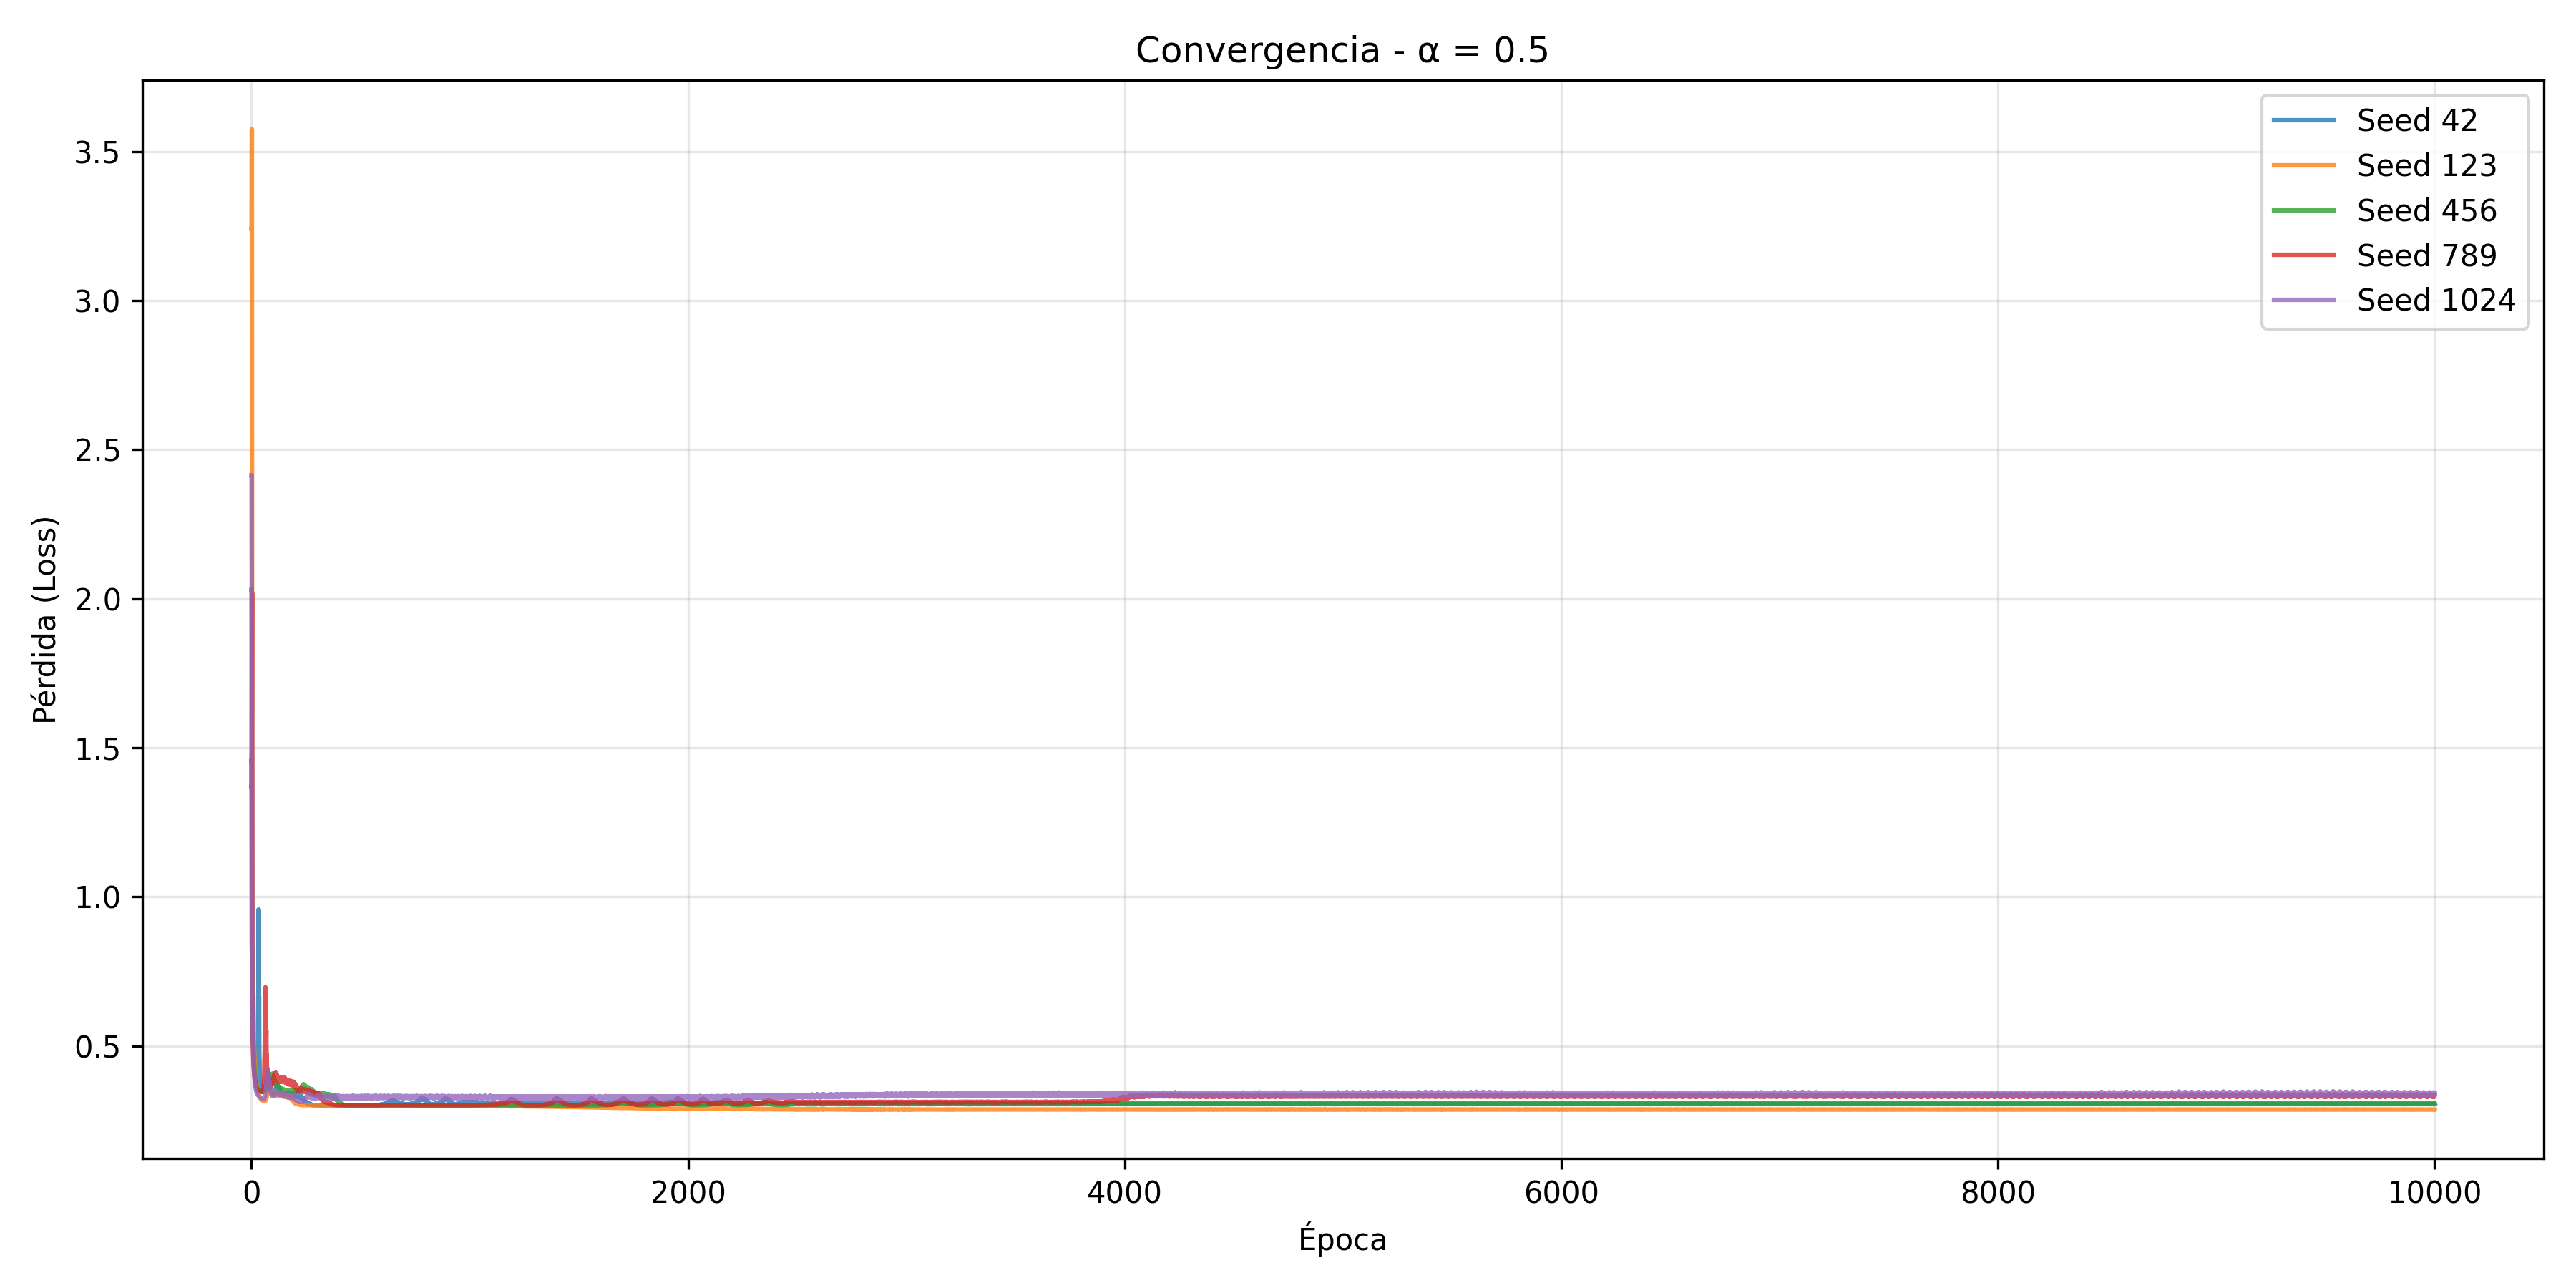
\includegraphics[width=0.95\textwidth]{../resultados/graficos/convergencia_alfa_0.5.png}
\caption{Convergencia del loss para $\alpha = 0.5$. Se observa una ca\'{i}da abrupta en las primeras 100 \'epocas seguida de un estancamiento. Las 5 semillas convergen a valores similares ($\sim 0.33$), indicando que la tasa grande ``aplana'' las diferencias de inicializaci\'{o}n.}
\label{fig:conv_0.5}
\end{figure}

\begin{figure}[H]
\centering
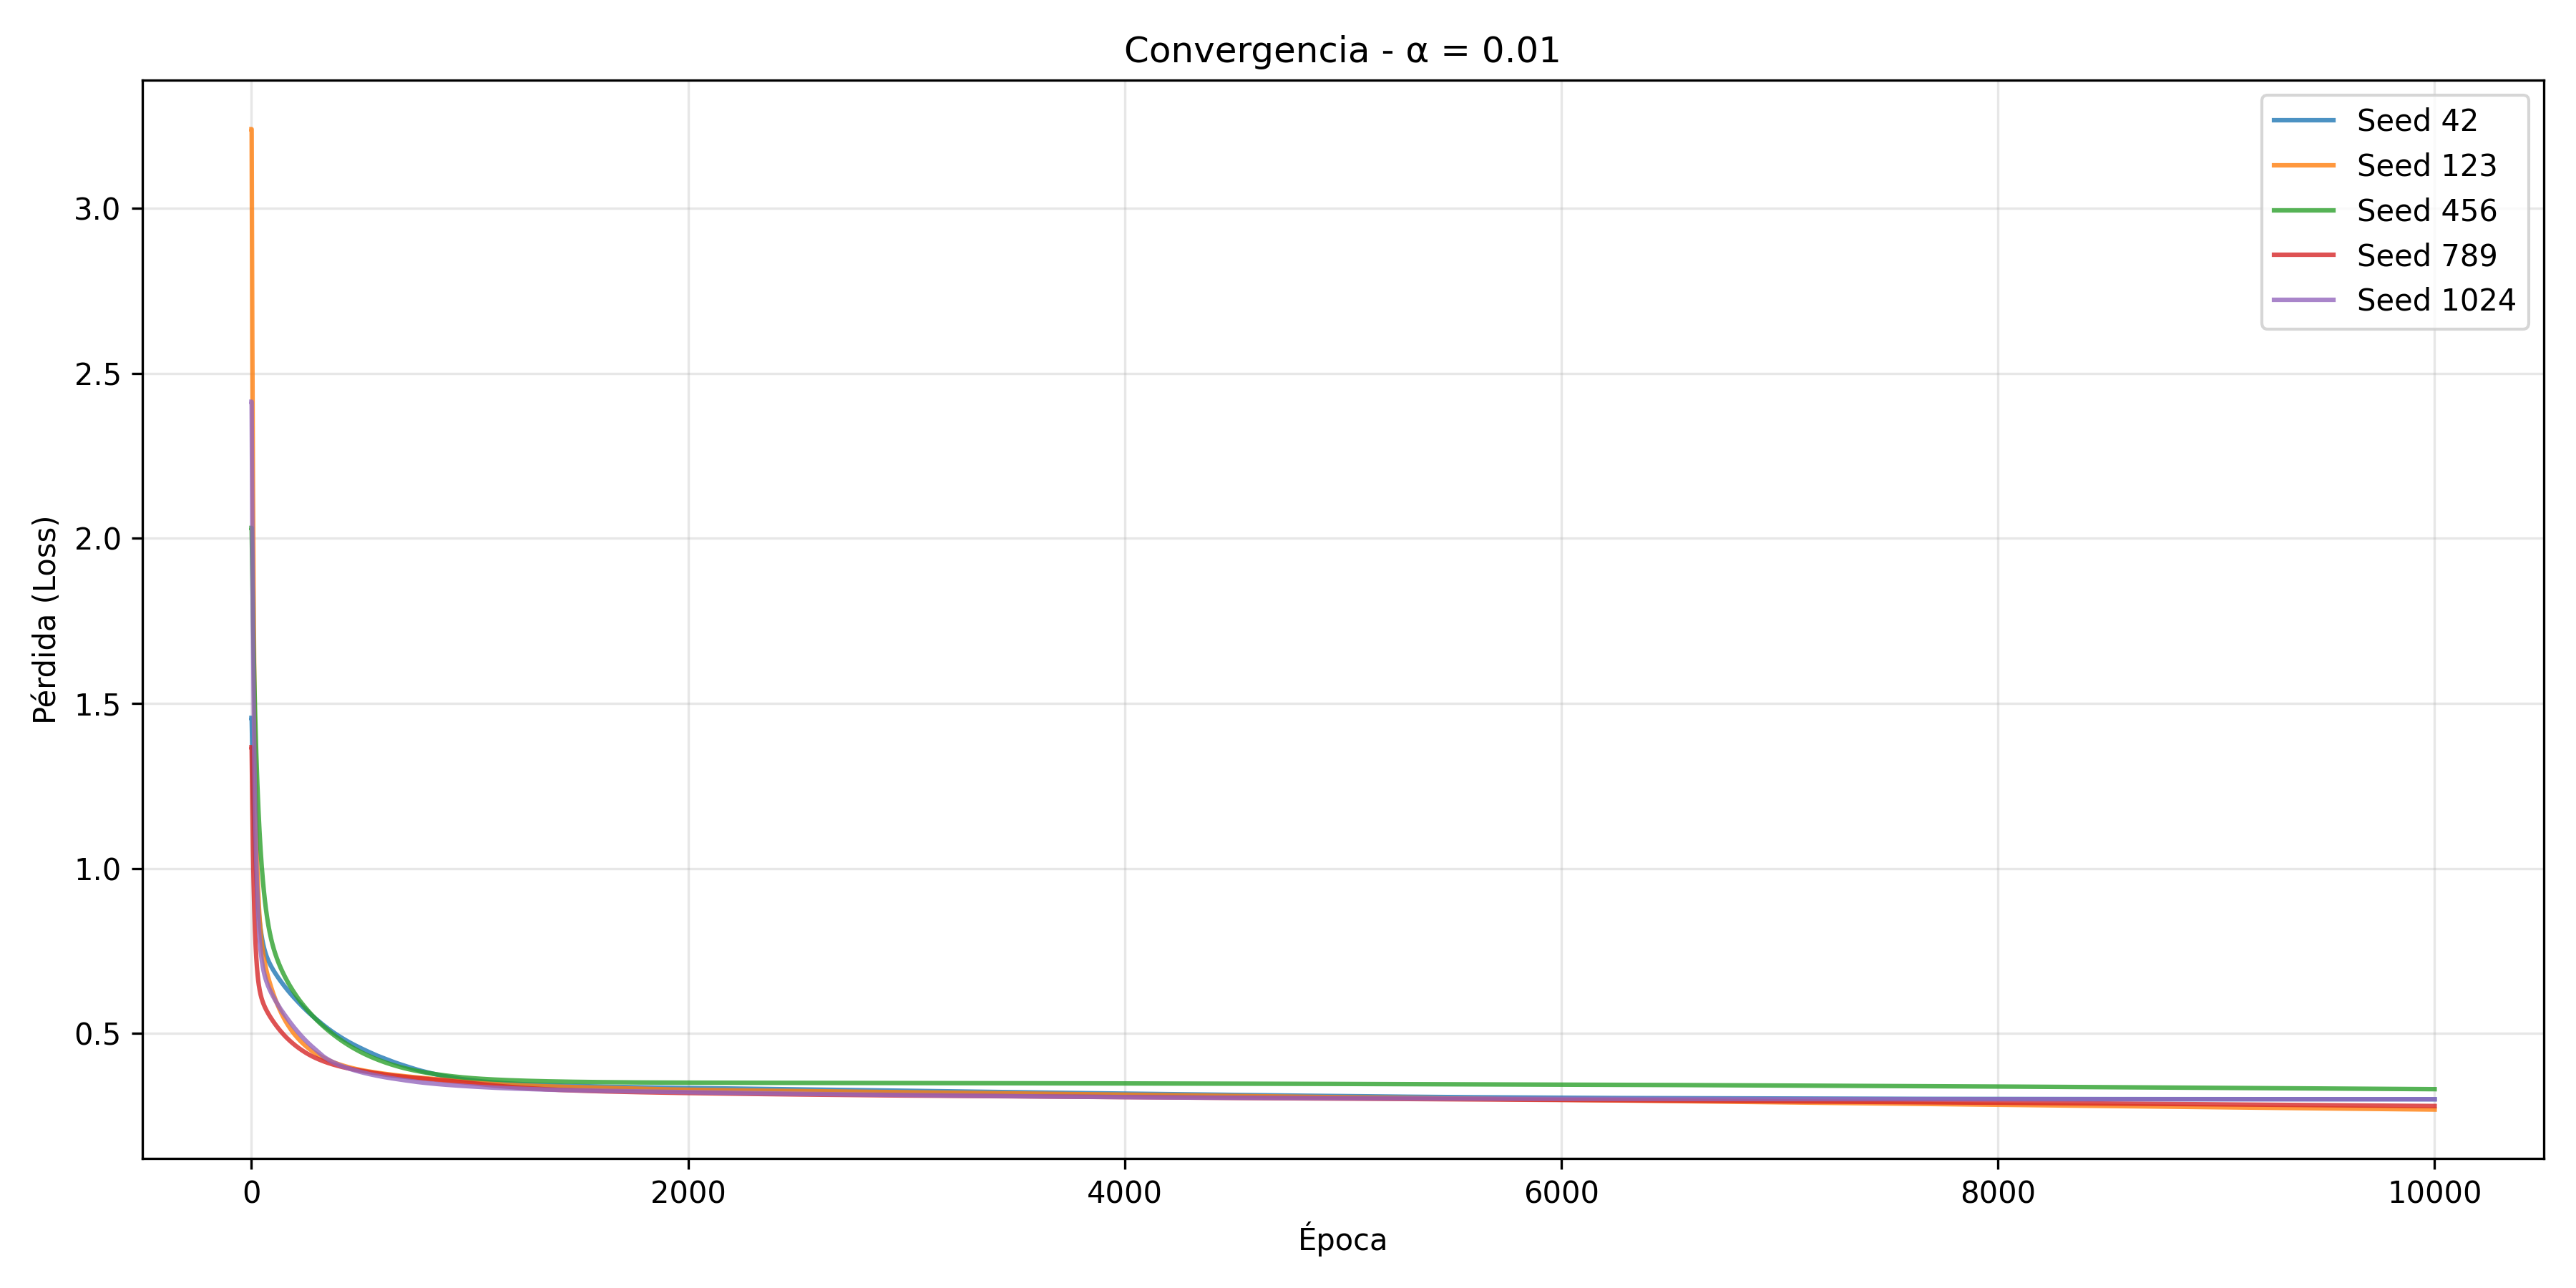
\includegraphics[width=0.95\textwidth]{../resultados/graficos/convergencia_alfa_0.01.png}
\caption{Convergencia del loss para $\alpha = 0.01$. Curvas suaves y mon\'{o}tonas decrecientes. La seed 123 alcanza el mejor resultado ($\sim 0.27$), mientras que la seed 456 se estanca en $\sim 0.33$.}
\label{fig:conv_0.01}
\end{figure}

\begin{figure}[H]
\centering
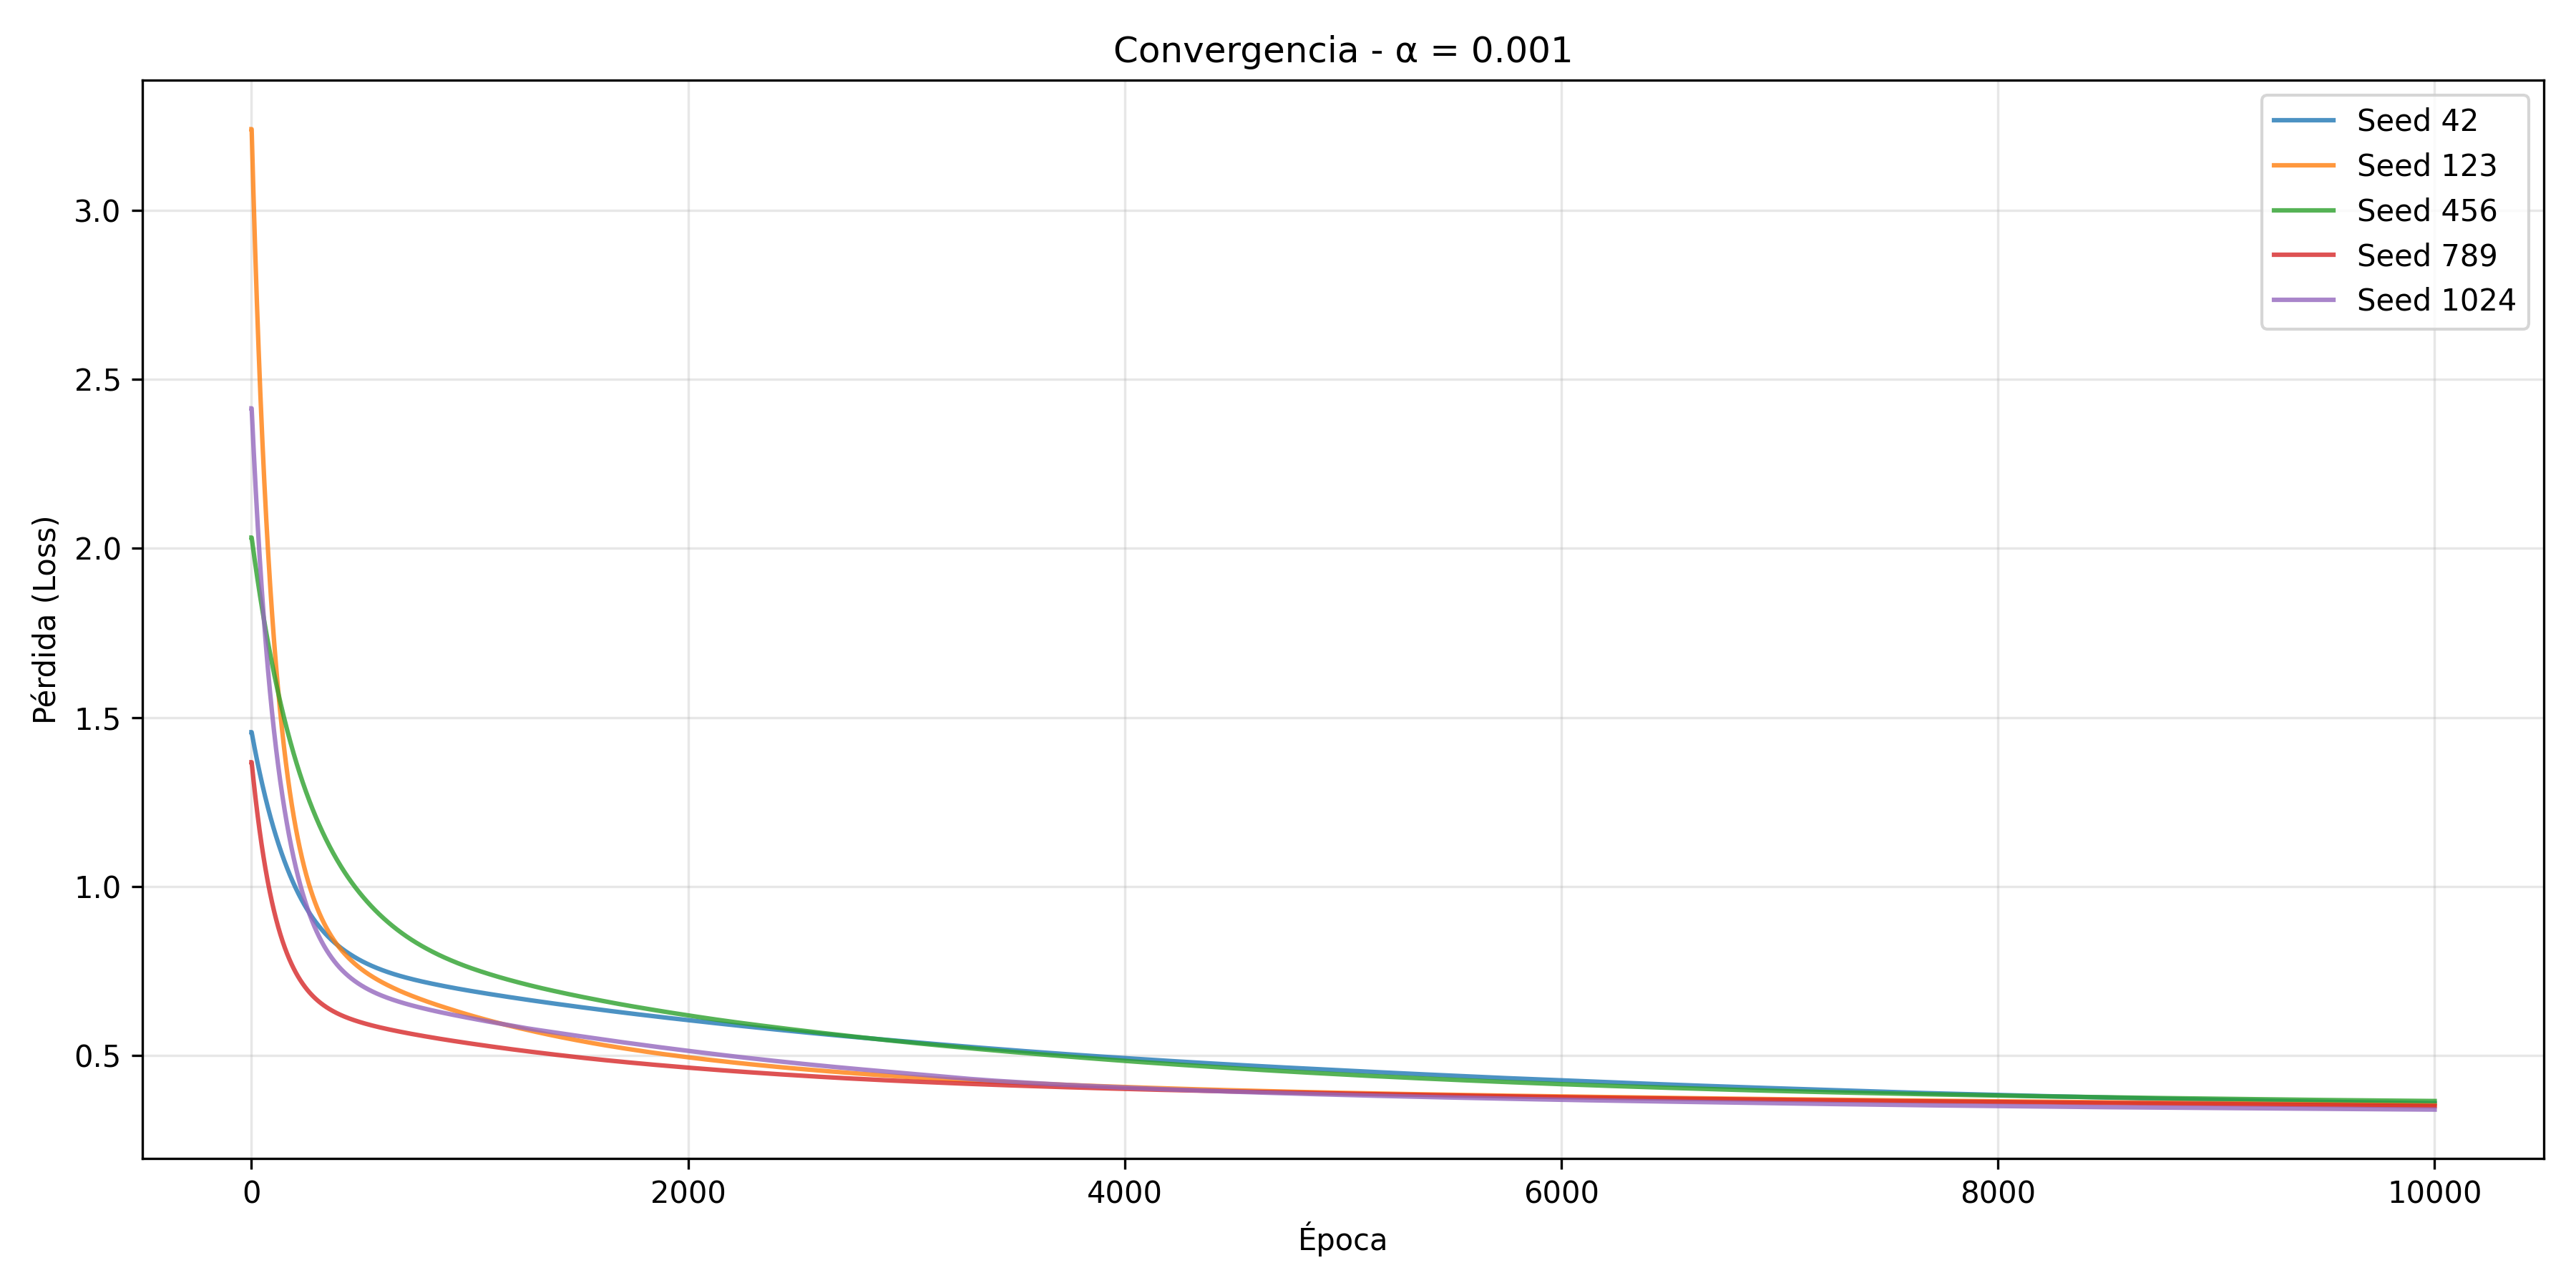
\includegraphics[width=0.95\textwidth]{../resultados/graficos/convergencia_alfa_0.001.png}
\caption{Convergencia del loss para $\alpha = 0.001$. La ca\'{i}da es muy lenta y las curvas a\'{u}n no se han estabilizado a las 10,000 \'epocas. Se requerir\'{i}an $\sim 50,000$ \'epocas para alcanzar el mismo loss que $\alpha = 0.01$.}
\label{fig:conv_0.001}
\end{figure}

\begin{figure}[H]
\centering
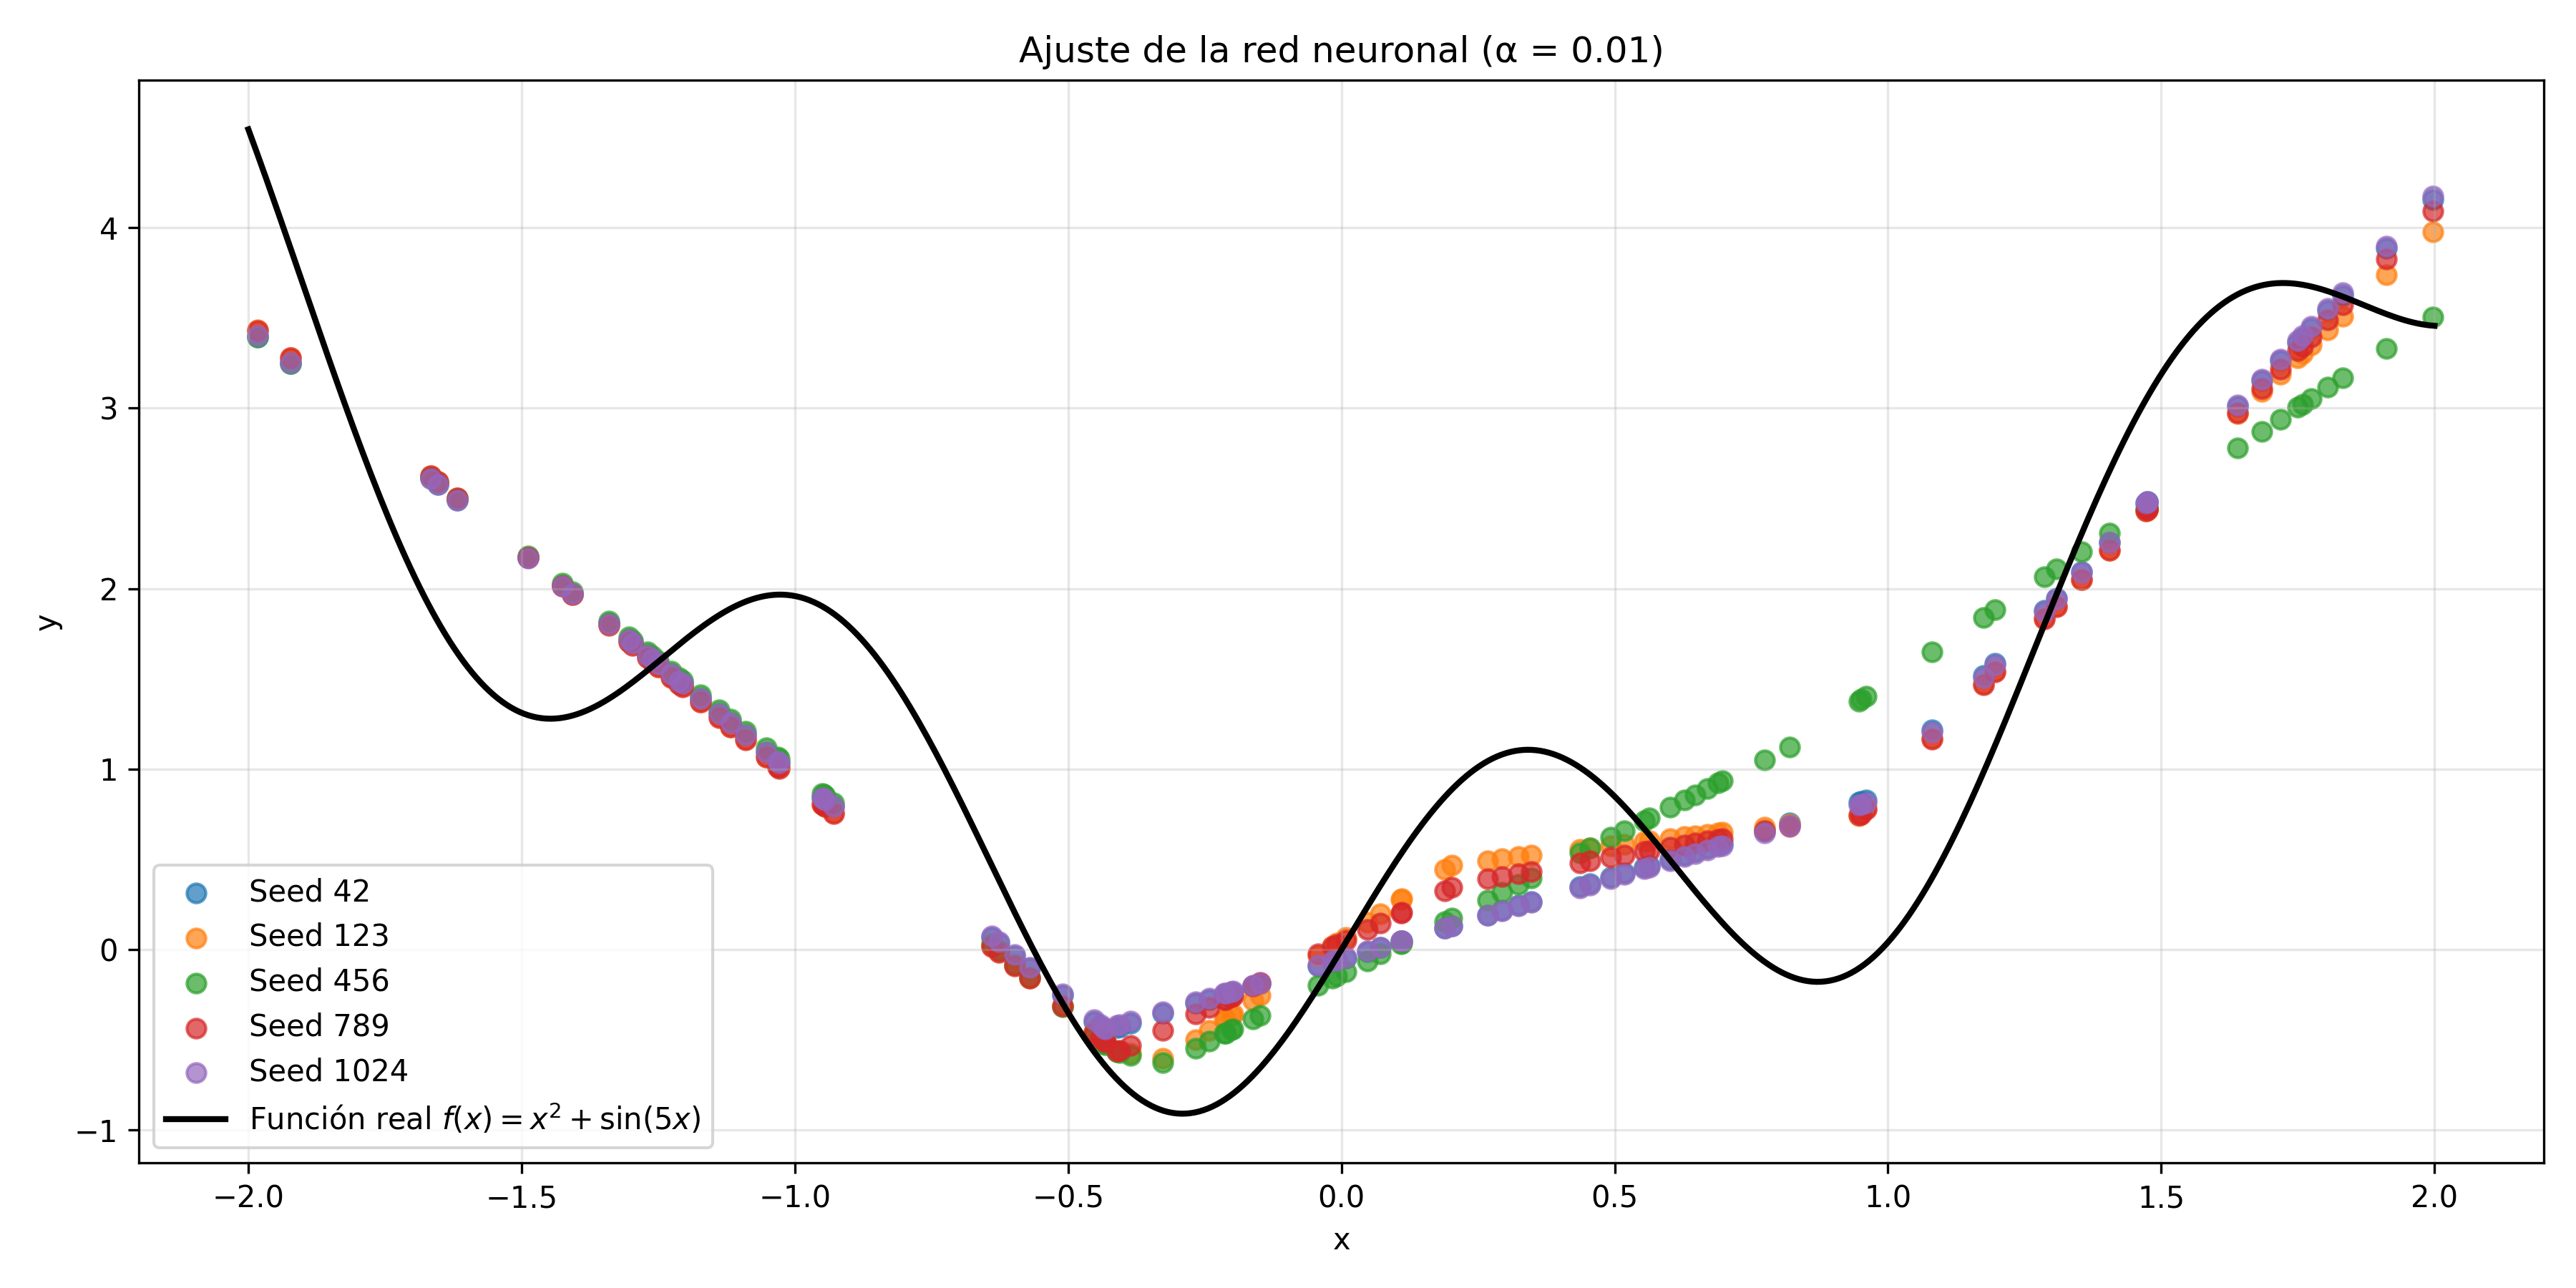
\includegraphics[width=0.95\textwidth]{../resultados/graficos/ajuste_alfa_0.01_todas_semillas.png}
\caption{Ajuste de la red neuronal para $\alpha = 0.01$. La l\'{i}nea negra muestra la funci\'{o}n real $f(x) = x^2 + \sin(5x)$. Los puntos de colores representan las predicciones de las 5 seeds. Se observa que la red captura la tendencia general pero tiene dificultades en las regiones de alta curvatura (cerca de $x = -1.5$ y $x = 1.8$).}
\label{fig:ajuste}
\end{figure}

% ---------- 5. ANALISIS MATEMATICO ----------
\section{An\'{a}lisis Matem\'{a}tico y Validaci\'{o}n}\label{sec:analisis}

\subsection{Derivaci\'{o}n Formal de los Gradientes}

Partiendo de la funci\'{o}n de costo $J = \frac{1}{2n}\sum_{i=1}^{n}(\hat{y}_i - y_i)^2$, aplicamos la Regla de la Cadena:

\subsubsection{Gradiente respecto a $w_2$}

\begin{align}
\frac{\partial J}{\partial w_2} &= \frac{\partial J}{\partial \hat{y}} \cdot \frac{\partial \hat{y}}{\partial w_2} \nonumber \\
&= \frac{1}{n}(\hat{y} - y) \cdot a_1 \nonumber \\
&= \delta_{\text{out}} \cdot a_1 \label{eq:deriv_w2}
\end{align}

\subsubsection{Gradiente respecto a $w_1$}

\begin{align}
\frac{\partial J}{\partial w_1} &= \frac{\partial J}{\partial \hat{y}} \cdot \frac{\partial \hat{y}}{\partial a_1} \cdot \frac{\partial a_1}{\partial z_1} \cdot \frac{\partial z_1}{\partial w_1} \nonumber \\
&= \delta_{\text{out}} \cdot w_2 \cdot f'(z_1) \cdot x \nonumber \\
&= \delta_{\text{hidden}} \cdot x \label{eq:deriv_w1}
\end{align}

donde $f'(z_1) = \begin{cases} 1 & \text{si } z_1 > 0 \\ 0 & \text{si } z_1 \leq 0 \end{cases}$ es la derivada de ReLU.

\subsection{Estabilidad Num\'{e}rica del Descenso de Gradiente}

La condici\'{o}n de estabilidad para el Descenso de Gradiente en una funci\'{o}n cuadr\'{a}tica es:

\begin{equation}\label{eq:estabilidad}
0 < \alpha < \frac{2}{\lambda_{\max}(H)}
\end{equation}

donde $H$ es la matriz Hessiana de $J$. Para $\alpha = 0.5$, es probable que se viole esta condici\'{o}n en regiones de alta curvatura, explicando las oscilaciones observadas en las primeras \'epocas.

\subsection{Impacto de la Inicializaci\'{o}n Aleatoria}

Los pesos se inicializan con distribuci\'{o}n normal $\mathcal{N}(0, 0.1)$. Diferentes semillas producen diferentes puntos de partida en el espacio de par\'{a}metros $\mathbb{R}^{2H+2}$, lo que lleva a diferentes m\'{i}nimos locales. Este fen\'{o}meno es inherente a la optimizaci\'{o}n no convexa y se mitiga parcialmente con:
\begin{itemize}
    \item M\'{u}ltiples ejecuciones con diferentes seeds.
    \item Tasa de aprendizaje adecuada para este problema siendo ($\alpha = 0.01$).
    \item Inicializaci\'{o}n cuidadosa (Xavier/He).
\end{itemize}

% ---------- 6. CONCLUSIONES ----------
\section{Conclusiones}\label{sec:conclusiones}

\begin{enumerate}
    \item Se implement\'{o} exitosamente una red neuronal con Backpropagation en C++17 con Eigen, siguiendo la metodolog\'{i}a \textbf{SDD} con especificaciones formales en Markdown y generaci\'{o}n de c\'{o}digo mediante Continue en VSCode.
    
    \item La derivaci\'{o}n manual de los gradientes (\textbf{zonas rojas} del taller) permiti\'{o} comprender en profundidad c\'{o}mo el error fluye desde la capa de salida hacia la capa oculta a trav\'{e}s de la Regla de la Cadena.
    
    \item El estudio de las 3 tasas de aprendizaje evidenci\'{o} el \textbf{trade-off fundamental} en el Descenso de Gradiente:
    \begin{itemize}
        \item $\alpha = 0.001$: convergencia segura pero extremadamente lenta.
        \item $\alpha = 0.01$: balance \'optimo entre velocidad y estabilidad.
        \item $\alpha = 0.5$: convergencia r\'{a}pida pero con riesgo de oscilaciones.
    \end{itemize}
    
    \item El an\'{a}lisis de las 5 semillas aleatorias confirm\'{o} la presencia de \textbf{m\'{i}nimos locales} en el paisaje de optimizaci\'{o}n no convexo. La variabilidad del loss final ($\sim 22\%$ para $\alpha = 0.01$) demuestra que la inicializaci\'{o}n aleatoria tiene un impacto significativo en la soluci\'{o}n final.
    
   \item La visualización del ajuste de la red reveló limitaciones estructurales en las regiones de alta curvatura de $f(x) = x^2 + \sin(5x)$. Este comportamiento se explica por tres factores fundamentales:
\begin{enumerate}
    \item \textbf{Aproximación lineal a trozos (ReLU):} La función de activación ReLU ($\max(0, z)$) fuerza a la red a aproximar la función objetivo mediante segmentos lineales. Con $H = 20$ neuronas en la capa oculta, la red solo puede generar un máximo de $H+1 = 21$ segmentos lineales (nudos). Dado que la segunda derivada de la función es $f''(x) = 2 - 25\sin(5x)$, las regiones de alta frecuencia ($\sin(5x)$) requieren una densidad de segmentos mucho mayor para capturar los cambios abruptos en la pendiente, resultando en un error de interpolación local.
    
    \item \textbf{Sesgo espectral (Spectral Bias):} Es un fenómeno conocido en redes neuronales que tienden a aprender primero los componentes de baja frecuencia (la tendencia global parabólica $x^2$) y mucho más lentamente los componentes de alta frecuencia (las oscilaciones de $\sin(5x)$). En 10,000 épocas, la red converge a un mínimo que minimiza el Error Cuadrático Medio (MSE) global, ``sacrificando'' el ajuste fino en los picos y valles locales.
    
    \item \textbf{Paisaje de optimización no convexo:} La función de pérdida de una red con ReLU es no convexa. Es altamente probable que el Descenso de Gradiente se haya estancado en un mínimo local subóptimo o en una región plana, donde algunas neuronas se ``murieron'' (Dead ReLU problem, donde $z \leq 0$ para todas las entradas), reduciendo efectivamente la capacidad de representación de la red por debajo de las 20 neuronas teóricas.
\end{enumerate}
\end{enumerate}
    

% ---------- REFERENCIAS ----------
\begin{thebibliography}{9}

\bibitem{goodfellow2016} Goodfellow, I., Bengio, Y., \& Courville, A. (2016). \textit{Deep Learning}. MIT Press. (Cap\'{i}tulo 6: Redes neuronales profundas).

\bibitem{bishop2006} Bishop, C. M. (2006). \textit{Pattern Recognition and Machine Learning}. Springer. (Cap\'{i}tulo 5: Redes neuronales).

\bibitem{rumelhart1986} Rumelhart, D. E., Hinton, G. E., \& Williams, R. J. (1986). \textit{Learning representations by back-propagating errors}. Nature, 323(6088), 533-536.

\bibitem{he2015} He, K., Zhang, X., Ren, S., \& Sun, J. (2015). \textit{Delving deep into rectifiers: Surpassing human-level performance on ImageNet classification}. Proceedings of the IEEE ICCV.

\bibitem{eigen} Eigen Documentation. \textit{Dense matrix and array manipulation}. \url{https://eigen.tuxfamily.org/dox/}

\bibitem{bottou2018} Bottou, L., Curtis, F. E., \& Nocedal, J. (2018). \textit{Optimization methods for large-scale machine learning}. SIAM Review, 60(2), 223-311.

\end{thebibliography}

\end{document}